\documentclass{article}
% Package to manage page layout
\usepackage[margin=1.5cm, includefoot, footskip=30pt]{geometry}

\setlength\parindent{0pt}
\setlength{\parskip}{1em}

%%%%%%%PACKAGES HERE%%%%%%%
\usepackage{amsmath}
\usepackage{hyperref}
\usepackage{standalone}
\usepackage{subcaption}
\usepackage{tikz}
\usepackage{booktabs}
\usepackage{minted}
\usepackage{multicol}
\usetikzlibrary{er,positioning, calc}

\definecolor{background}{RGB}{5, 66, 81}
\usemintedstyle{tango}
%%%%%%%%%%%%%%%%%%%%%%%%%%%
\title{Literature review paper for the iterated prisoner's dilemma.}
\author{Nikoleta E. Glynatsi}
\date{2016}

\begin{document}

\maketitle

\section{Introduction}\label{section:introduction}

The emergence of cooperation is a topic of continuing and public interest
for social~\cite{capraro2014, gracia2012},
biological~\cite{Douglas2011}
and ecological sciences~\cite{Godfray1992,Krama2012,Milinski1987,Wilkinson1984}.
Cooperation is essential for evolution but according to Darwin’s theory 
it is not always easy to achieve. The game called the prisoner's
dilemma offers a theoretical framework for studying the emergence of
altruist behaviour. Collecting data from 5 sources shows that more than 1170 papers
related to the prisoner's dilemma have been published since it's origin.

In this work an extensive literature review will be presented. In addition, 
an introduction to the prisoner's dilemma is given in Section~\ref{section:prisoners_dilemma}
and some major pieces of work will be discussed in Section~\ref{section:timeline}.
In Section~\ref{section:analysis} a comprehensive data set of literature
regarding the prisoner's dilemma will be presented and analysed.

\section{The Prisoner's Dilemma}\label{section:prisoners_dilemma}

The prisoner's dilemma a two player no-cooperative game where the decisions
of the players are made simultaneously and independently. Both players can
choose between cooperation (\textbf{C}) or defection (\textbf{D}).

The fitness of each player is influenced by its own behaviour, and the behaviour
of the opponent. If both players choose to cooperate, both do better
than if both defect. However, a player has the temptation to deviate. If a
player was to defect while the other cooperates, the defector receives
more than if both had cooperated. The reward for mutual cooperation is \(R\)
units, for a mutual defection they receive \(P\), and for cooperation-defection,
the cooperator receives \(S\) where the defector receives \(T\). Thus, the game's
payoffs are given by,

\begin{equation} \label{eq:the_pd_payoffs}
    \begin{pmatrix}
    R & S \\ T & P
    \end{pmatrix}
\end{equation}

where \(T > R > P > S \) and \(2R > T + S\) are the conditions for a dilemma
to exist. Due to rational behaviour and the knowledge that an individual is tempted
to defect the game's equilibrium lies at a mutual defection and both players
receive a payoff of \(P\). Thus, the unbeatable strategy for the prisoner's dilemma
is \textbf{D}.

However, when the game is studied in a manner where prior outcomes matter, the 
defecting choice is no longer necessarily the unbeatable choice. The repeated 
form of the game is called the iterated prisoner's dilemma and now players 
interact more than just once.

In Section~\ref{section:timeline} it will be discussed how it was proven that
the iterated prisoner's dilemma leaves room for cooperation. The prisoner's
dilemma has attracted much attention and that's shown in Figure
\ref{fig:timeline}. Figure~\ref{fig:timeline} illustrates the number of 
publications on the prisoner's dilemma per year from the following sources:

\begin{multicols}{3}
    \begin{itemize}
        \item arXiv;
        \item PLOS;
        \item IEEE;
        \item Nature;
        \item Springer.
    \end{itemize}
\end{multicols}

The choice of sources is due to the fact that they have an open access API
which will be discussed in more detail in Section~\ref{section:analysis}. %TODO add some information
The data collection and the open source library used to generate the time plot 
will be described more comprehensively in Section~\ref{section:analysis}.
There are various specific timepoints that will be discussed in Section
\ref{section:timeline}.

\begin{figure}[!htbp]
    \centering
    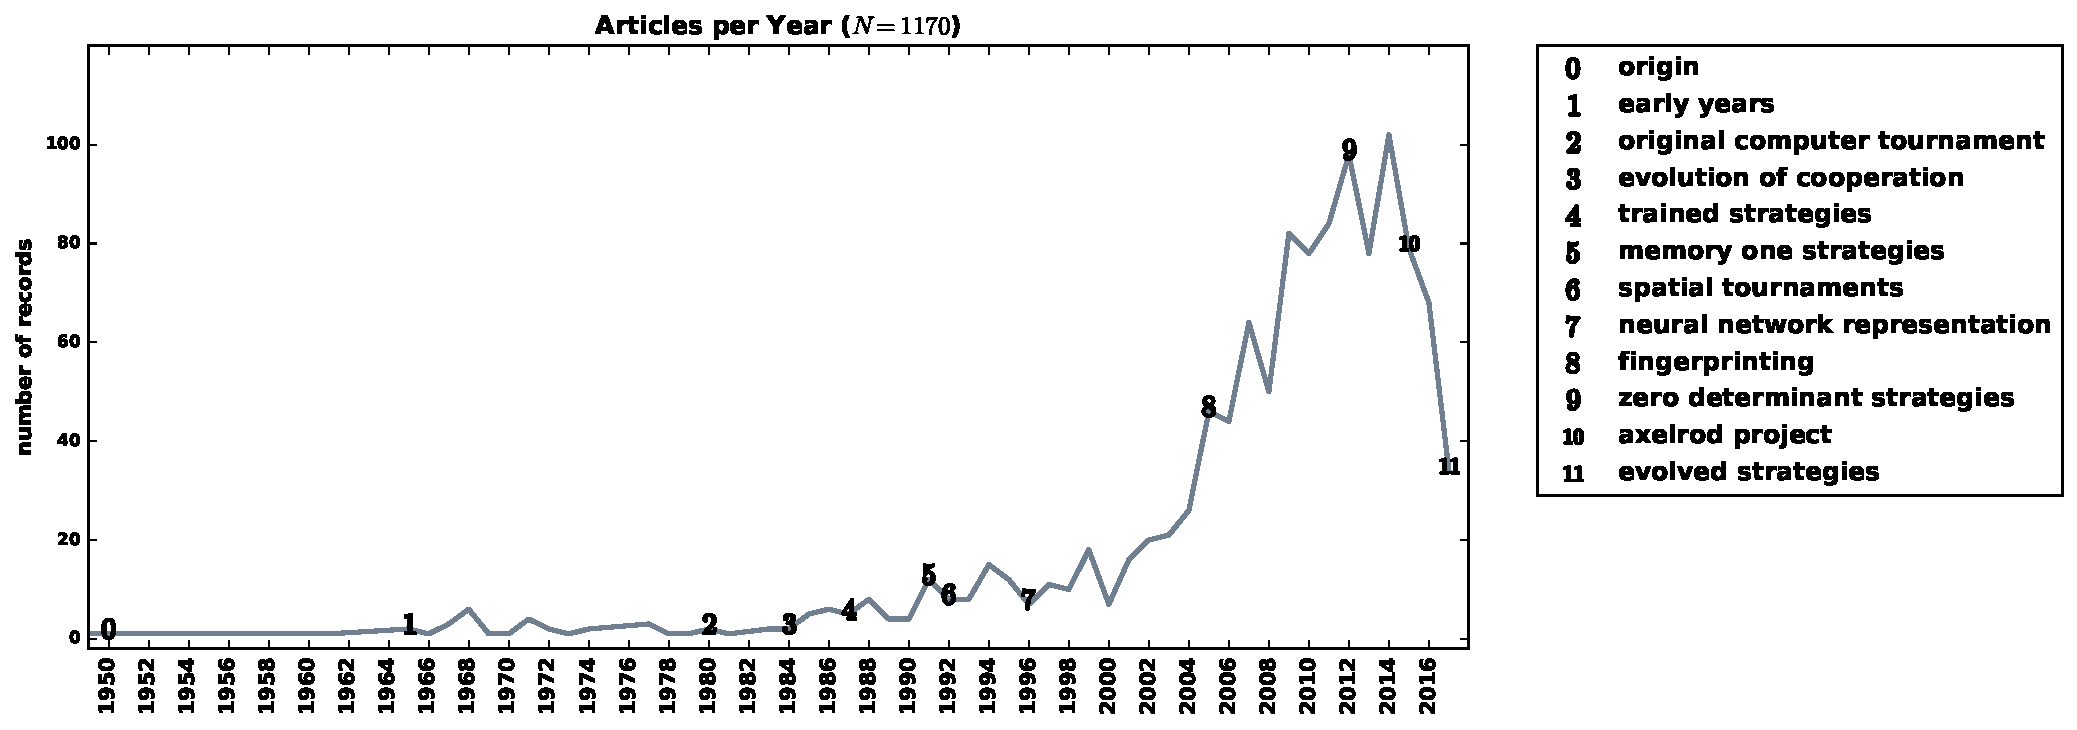
\includegraphics[width=\textwidth]{assets/images/timeline.pdf}
    \caption{\label{fig:timeline} A timeline highlighting the milestones of the 
    prisoner's dilemma.}
\end{figure}

\section{Timeline}\label{section:timeline}

\subsection{Origin and the 60's}

The origin of the prisoner's dilemma go back to 1950s in early experiments
conducted in RAND~\cite{Flood1958} to test the applicability of games
described in~\cite{VonNeumann1944}. In~\cite{Flood1958} the two player game was
introduced but the name behind the game was given later the same year. 
A. W. Tucker, the PhD advisor of John Nash, in an attempt to delivery the game
with a story during a talk used prisoners as players and the game is known as 
the prisoner's dilemma ever since~\cite{Tucker1983}.

The study of the prisoner's dilemma has attracted people from various fields
across the years. An early figure within the field is Professor Anatol Rapoport,
a mathematical psychologist, whose work focused on peacekeeping.
In his early work~\cite{rapoport1965} Rapoport conducted experiments using humans
to simulate a play of the prisoner's dilemma. Experimental groups were not been
used only by Rapoport but it was a common mean of studying the game
\cite{Evans1966, Gallo1968, Lutzker1961, Mack1971, Sensenig1972} and are still
being use to date. %TODO reference a good article with human studies.

Several experiments explored the conditions under which altruist behaviour emerges
in human societies. Conditions that were studied include, the gender~\cite{Evans1966,
Lutzker1961, Mack1971} of individuals, the representation of the game
\cite{Evans1966}, the distance between players~\cite{Sensenig1972}, the start effect
\cite{Tedeschi1968} and whether the experimenter has been biaised~\cite{Gallo1968}.

Though the aspects of representation, distance and starting effect were proven 
in the 60's to have a significant effect on the cooperating ratio of the 
individuals, the aspect of gender was found to be insignificant. An interesting
result has been the effect of the representation, or the  explanation of the game 
itself. It shows that when people are playing the prisoner' dilemma 
any minor change in the presentation of the game can have an effect on their
interpretation of the game. 

Other experiments focused on analysing the play of a test subject. Researchers believed
that they could identify an unbeatable strategy to play the game. Inspired by 
the work of Rapoport and the idea that AI was now being trained to play a 
game of chess the political scientist Robert Axelrod performed
the first ever computer tournament, known to the author, of the iterated 
prisoner's dilemma~\cite{axelrod2012, Axelrod1981}.

\subsection{Axelrod's Tournaments}\label{subsection:axelrods_tournament}

In 1980~\cite{axelrod1980a} a computer tournament of the iterated prisoner's
dilemma took place. R. Axelrod invited 14 participants to submit a strategy written
in the programming languages Fortran or Basic; the names of the attendants were
the following,

\begin{multicols}{2}
    \begin{enumerate}
        \item T Nicolaus Tideman and Paula Chieruzz;
        \item Rudy Nydegger;
        \item Bernard Grofman;
        \item Martin Shubik;
        \item Stein and Anatol Rapoport;
        \item James W Friedman;
        \item Morton Davis;
        \item Jim Graaskamp;
        \item Leslie Downing;
        \item Scott Feld;
        \item Johann Joss;
        \item Gordon Tullock;
        \item Name not given;
    \end{enumerate}
\end{multicols}

Each strategy played against all the 14 opponents, itself and a player that played
randomly a match of 200 turns. This topology is called round robin and is the 
equivalent of a complete graph. The tournament was repeated \(5\) times to
reduce variation in the results. Each participant knew the exact length of the
matches and had access to the full history of each match. Furthermore, Axelrod
performed an preliminary tournament and the results were known to the participants.
The payoff values used where \(R=3, P=1, T=5\) and \(S=0\). These values are
commonly used in the literature and unless specified will be the values used in
the rest of the work described here. 

The winner of the tournament was determined by the total average score and not by
the number of matches won. The strategy that was announced the winner was
submitted by Rapoport and was called \textbf{Tit For Tat}. Tit for Tat, is a 
strategy that always cooperates on the first round and then mimics the opponent's
previous move. 

Examples of Tit for Tat interacting with deterministic opponents are given by 
Tables~\ref{table:tft_vs_c}, \ref{table:tft_vs_d}, \ref{table:tft_vs_a}. 
The opponents are, \textbf{Cooperator} a strategy that always cooperates, 
\textbf{Defector} an opponent that always defects and \textbf{Altenator} a 
player who alternates between cooperating and defecting.

\begin{table}[!hbtp]
    \begin{center}
    \begin{tabular}{lcc}
        \toprule
        Turns & Tit for Tat & Cooperator\\
        \toprule
        1 & C & C\\
        2 & C & C\\
        3 & C & C\\
        $\vdots$ & $\vdots$ & $\vdots$ \\
        200 & C & C \\
        \bottomrule
    \end{tabular}
    \caption{Tit for Tat example match against Cooperator}\label{table:tft_vs_c}
    \end{center}
\end{table}

\begin{table}[!hbtp]
    \begin{center}
    \begin{tabular}{lcc}
        \toprule
        Turns & Tit for Tat & Defector\\
        \toprule
        1 & C & D\\
        2 & D & D\\
        3 & D & D\\ 
        $\vdots$ & $\vdots$ & $\vdots$ \\ 
        200 & D & D \\
        \bottomrule
    \end{tabular}
    \caption{Tit for Tat example match against Defector}\label{table:tft_vs_d}
\end{center}
\end{table}

\begin{table}[!hbtp]
    \begin{center}
    \begin{tabular}{lcc}
        \toprule
        Turns & Tit for Tat & Altenator\\
        \toprule
        1 & C & C\\
        2 & C & D\\
        3 & D & C\\ 
        $\vdots$ & $\vdots$ & $\vdots$ \\ 
        200 & C & D \\
        \bottomrule
    \end{tabular}
    \caption{Tit for Tat example match against Altenator}\label{table:tft_vs_a}
\end{center}
\end{table}

The results of the first tournament was filled with surprises. Tit for Tat won 
but was the simplest strategy of all. Tit for Tat managed to defeat even
entrants that tried to improve on Tit for Tat after the preliminary tournament.

Axelrod explained the reasons behind Tit for Tat's success. The top eight ranked
strategies have been strategies that never defected on the first round, thus they were
`nice'. Amongst those top strategies the results were determined by just two 
of the other seventh rules. Those strategies were described as kingsmakers and they 
were the strategies submitted by Grofman and Graaskamp. The final property
that was described to have affect Tit for Tat's performance compared to the 
rest strategies was `forgiveness'. Tit for Tat punished it's opponent for a 
defection but just once.

Axelrod was the first to speak about `niceness' and `forgiveness' as properties
of a winning strategy for the iterated prisoner's dilemma. To further test the
robustness of the results Axelrod performed a second tournament~\cite{axelrod1980b}.
A total of 63 participants submitted strategies for the second tournament, 
their names were the following,

\begin{multicols}{3}
    \begin{enumerate}
        \item Gail Grisell;
        \item Harold Rabbie;
        \item James W Friedman;
        \item Abraham Getzler;
        \item Roger Hotz;
        \item George Lefevre;
        \item Nelson Weiderman;
        \item Tom Almy;
        \item Robert Adams;
        \item Herb Weiner;
        \item Otto Borufsen;
        \item R D Anderson;
        \item William Adams;
        \item Michael F McGurrin;
        \item Graham J Eatherley;
        \item Richard Hufford;
        \item George Hufford;
        \item Rob Cave;
        \item Rik Smoody;
        \item John Willaim Colbert;
        \item David A Smith;
        \item Henry Nussbacher;
        \item William H Robertson;
        \item Steve Newman;
        \item Stanley F Quayle;
        \item Rudy Nydegger;
        \item Glen Rowsam;
        \item Leslie Downing;
        \item Jim Graaskamp and Ken Katzen;
        \item Danny C Champion;
        \item Howard R Hollander;
        \item George Duisman;
        \item Brian Yamachi;
        \item Mark F Batell;
        \item Ray Mikkelson;
        \item Craig Feathers;
        \item Fransois Leyvraz;
        \item Johann Joss;
        \item Robert Pebly;
        \item James E Hall;
        \item Edward C White Jr;
        \item George Zimmerman;
        \item Edward Friedland;
        \item X	Edward Friedland;
        \item Paul D Harrington;
        \item David Gladstein;
        \item Scott Feld;
        \item Fred Mauk;
        \item Dennis Ambuehl and Kevin Hickey;
        \item Robyn M Dawes and Mark Batell;
        \item Martyn Jones;
        \item Robert A Leyland;
        \item Paul E Black;
        \item T Nicolaus Tideman and Paula Chieruzz;
        \item Robert B Falk and James M Langsted;
        \item Bernard Grofman;
        \item E E H Schurmann;
        \item Scott Appold;
        \item Gene Snodgrass;
        \item John Maynard Smith;
        \item Jonathan Pinkley;
        \item Anatol Rapoport.
    \end{enumerate}
\end{multicols}

All the participants knew the results of the previous tournament. The rules 
were similar to those of the first tournament with only one exception;
the number of turns was not specified. A probabilistic ending tournament was
meant to be used. In a probabilistic ending tournament each match has probability 
of ending after each turn. This is  also refereed as `shadow of the future'
\cite{axelrod1988}. 

However, the tournament was not a probabilistic ending one. A fixed probability 
of  0.0036 was chosen as a chance of ending a match with each given move. The
value was chosen so that the expected median length of a match would be 200
turns. The topology was of a round robin and each pair of players was matched 
5 times. The length of the matches was determined once by drawing a random sample.
Each of the five matches had a length of 63, 77, 151 and 308.

The results of the tournament once again came as a surprise. Tit for Tat was the
simplest submission in the second tournament and won the second tournament as well.
Tit for Tat provided proof that reciprocity behaviour can allow cooperation
to emerge in the iterated prisoner's dilemma game. In~\cite{Axelrod1981}
the main conclusions indicating strong performance was:

\begin{itemize}
    \item that it start of by cooperating
    \item it would forgive it's opponent after a defection
    \item after opponents identified that they were playing Tit for Tat choose
    to cooperate for the rest of the game.
\end{itemize}
%The strategies of the second tournament where bias due the first tournament. Discuss with V. 
%TODO add better conclusion on Axelrod's work

Though a full explanation of all 14 strategies in given in~\cite{Axelrod1981}
the same does not hold for all 63 strategies of the second tournament~\cite{Axelrod1981}.
The author mainly focuses on the high ranked participants. However, the source 
code for of the strategies be found on Axelrod's personal website~\cite{fortan_code}.
The code has been written by Axelrod and several other contributors in the programming 
languages Fortran or Basic. The strategies written in Basic were translated to 
Fortran before the tournament. The source code includes the code only for the
strategies and not for creating and performing the tournament.

The code for the winning strategy Tit for Tat is illustrated in Figure
\ref{fig:tit_for_tat_fortran}.

\begin{figure}[!hbtp]
    \centering
    \begin{minted}
        [
        autogobble=true,
        framesep=2mm,
        fontsize=\normalsize,
        ]
        {fortran}
    FUNCTION K92R(J,M,K,L,R, JA)
C BY ANATOL RAPOPORT
C TYPED BY AX 3/27/79 (SAME AS ROUND ONE TIT FOR TAT)
c replaced by actual code, Ax 7/27/93
c  T=0
c   K92R=ITFTR(J,M,K,L,T,R)
      k92r=0
      k92r = j
c test 7/30
c   write(6,77) j, k92r
c77   format(' test k92r. j,k92r: ', 2i3)
      RETURN
      END
    \end{minted}
    \caption{\label{fig:tit_for_tat_fortran} Source code for Tit for Tat in Fortran.
    Provided by~\cite{fortan_code}.}
\end{figure}

Unfortunately, the source code of the first tournament is not 
available as stated in Axelrod's personal website~\cite{fortan_code}.

Other successful strategies from Axelrod's tournament that can been seen 
in literature to date are, 

\begin{itemize}
    \item \textbf{Grudger} is a strategy that will cooperate as long as the 
    opponent does not defect. The name Grudger was give to the strategy in~\cite{Li2014}.
    Though the strategy goes by many names in the literature such as, 
    Spite~\cite{Beaufils1997}, Grim Trigger~\cite{Banks1990} and Grim~\cite{Van2015}.
    \item etc
\end{itemize}

% The success of Tit For Tat was very soon known world wide and several researchers
% focused their work on the strategy ever since~\cite{Douglas2011, Krama2012, Milinski1987}.
%TODO keep adding references of future works featuring Tit for Tat.
%TODO add a sentence for each

% Following the successful work of computer tournaments many researchers have sought
% to understand which strategies are dominant when playing the iterated prisoner's
% dilemma. These strategies vary from deterministic to more complex ones.
% Strategies can rely on the history of the game, the length of the matches or 
% choose to rely on none of above. The size of history a strategy takes into account
% is refereed to as the memory size of the strategy. 
% %TODO reference an article that refers to memory size.
\subsubsection{Mis implementation}

Success often comes with criticism. Axelrod's tournaments assumed that
each player has perfect information of the opponent's actions. In real life
situations this is not always the case. Colleagues' interactions often suffer from
measures of uncertainty. In the original tournaments there was no possibility of
mis implementation or misunderstanding. These stochastic variations are refereed
to as \textbf{noise} and \textbf{mis perception}. Noise is the concept of flipping
one's move based on a given probability. On the contrary, mis perception is the
probability that the opponent's current move is flipped before being recorded.
Noise will flip a player's action  and it will be recorded correctly in the history
where mis perception will not have an effect on the player's move but it will be
recorded wrong~\cite{Hoffmann1998}.
%TODO break this down

The performance of Tit for Tat was proven to suffer from such stochasticity in
the tournament environment, especially against itself~\cite{Bendor1991,Godfray1992,
Molander1985, Nowak1992, Wolfgang2006}. If two strategies playing Tit for Tat were
to compete against each other in a noisy environment the strategies will get 
a series of unwanted defections. In a non noisy environment
the two strategies would have been cooperating for the entire match.
An interesting result was introduced by~\cite{Molander1985}. Molander stated
that if two strategies playing Tit for Tat meet in a noisy match the average
payoff that a strategy will receive will be the same as that of a Random player
(with probability \(0.5\) of cooperating). 

In~\cite{Bendor1991} a similar tournament to that of Axelrod was performed 
but this time noise was used. Bendor invited academics to submit strategies 
to participate in his tournament. A total of thirteen strategies were used 
including already existed strategies such as Tit for Tat and \textbf{Tit for 2 
Tats}. The results showed that Tit for Tat performed purely placing eight in
the tournament. Bendor stated that a more forgiving strategy was needed, in his
tournament a strategy called \textbf{Nice and Forgiving} ranked first.

The work of~\cite{Nowak1992} following a similar approach agreed with this result.
In~\cite{Nowak1992}, the space of re-active strategies was explored in a noisy
environment. The strategy that was performing the best in that environment was
the re-active strategy known as \textbf{Generous Tit for Tat}. A reactive 
strategy is a strategy that consider only the past move of the opponent, but 
they will be discussed later on in more detail. Generous Tit for Tat, attracted
attention as it was a generous variant of the famous strategy Tit for Tat able
to withstand noisy environments.

The author published yet another paper a years later~\cite{Nowak1993} introducing another
interesting player. The new strategy had the tolerance of Generous Tit for Tat 
but also the capability of resisting and invading an all-out cooperators population
was. The strategy is called \textbf{Pavlov},
and is based on the fundamental behavioural mechanism win-stay, lose-shift.
The strategy starts off with a \textbf{C}, then Pavlov will repeat it's last
move it was awarder with by \(R\) or \(T\) but will shift if punished by \(P\) or
\(S\).

% The pioneer work of computer tournaments in the iterated prisoner's dilemma
% sparked an interest within the field and several studies and approaches are
% discussed in the following sections.

\subsection{Strategies Stability}

So far it has been discussed that a strategy's dominance is tested through
the performance of the strategy in a tournament against other strategies.
But is the overall success of a strategy based only on it's performance in a 
round robin tournament or should it be checked through other ways as well?

Following his initial tournaments Axelrod performed an `ecological' tournament
in 1981~\cite{Axelrod1984}. In~\cite{Axelrod1984}, the set of strategies from 
Axelrod's second tournament was used to perform the ecological tournament. The 
63 strategies interacted generation after generation to a round robin competition
where their frequencies were proportional to their payoff in the previous round.
The ecological approach is based on the payoff matrix of the tournament. The
highest performing strategies are adapted by lower scoring individuals
within a fixed population. Over time a strategy takes over the population.
Figure~\ref{fig:ecological.tournament} demonstrates an example of the
natural selection proceeder.

The ability of strategies to be favoured under natural selection and their 
ability to withstand invasion from other strategies soon became an new measure 
of performance; refereed to as the stability of a strategy.

\begin{figure}[!hbtp]
    \centering
    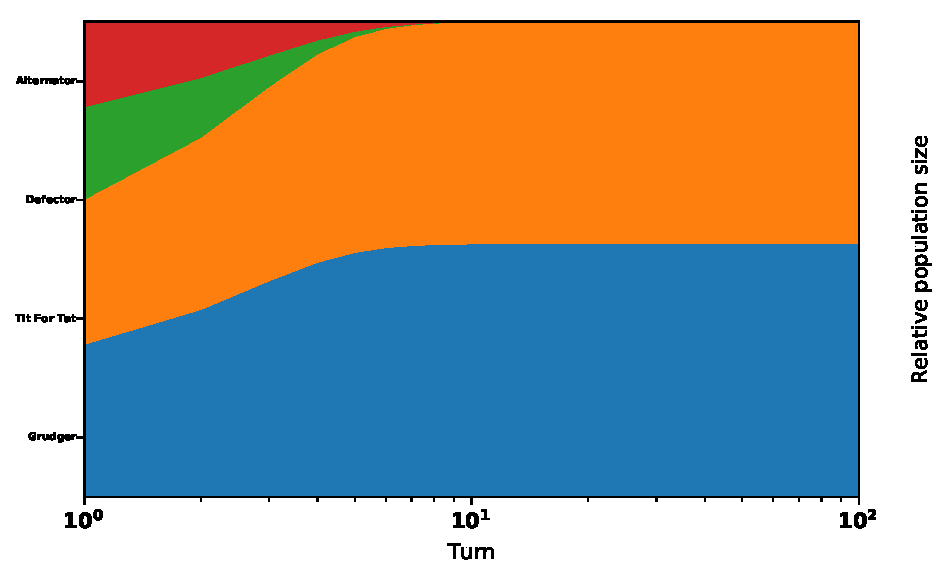
\includegraphics[width=.6\textwidth]{./assets/images/ecological.pdf}
    \caption{System evolving over time based on natural selection using
    \cite{axelrodproject}.}
    \label{fig:ecological.tournament}
\end{figure}
%TODO I've been fighting with the yticks fontsize. Need to ask Geraint.

In~\cite{Axelrod1981}, the results showed that in a homogeneous
population of Tit for Tat invasion by mutant strategies was not successful.

The results of~\cite{Boyd1987} argued that no pure strategy is evolutionary
stable in the iterated prisoner's dilemma. This was not proven analytically, instead
a series of examples using strategies such as Tit for Tat, Suspicious
Tit for Tat and Defector where explored; a very constrained set of strategies.

The results were questioned by~\cite{May1987}, stating that much was
still no fully explored and more research had to be put into the results.
Another attempt to explore stability of strategies in the prisoner's dilemma
was done in~\cite{Boyd1989}. This time exploring the results in a noisy
environment, but similarly a analytical proof was not achieved.

\subsection{Spatial tournament}

An extension to the natural selection was introduced in the 1992~\cite{Nowak1992b},
recommending a different type of topology. A population of two deterministic
strategies, Defector and Cooperator, were placed on a a two dimensional square array
where the individuals could interact only with the immediate neighbours.
The number of immediate neighbours could be either, fourth, six or eight. As
shown in Figure~\ref{fig:topologies}. The authors claimed that the essential
results remain true of all topologies; the results also hold whether self interactions
are taken into account.

Thus each cell of the lattice is occupied by a \textbf{C} or a \textbf{D} and in
each generation step each cell owner interacts with its immediate neighbours and
play the game. The score of each player is the sum of the overall games the player
competed in. At the start of the next generation, each lattice cell is occupied by the
player with the highest score among the previous owner and the immediate
neighbours. Nowak and all created this model where the model parameter
has been the temptation payoff denoted as \(b\). Thus \(T=b\). For 
different values of the parameter \(b\) it was shown that cooperators and
defectors can persist together indefinitely. This topology is refereed to as
spatial topology.

\begin{figure}[!hbtp]
\centering
    \begin{subfigure}{.25\textwidth}
        \includestandalone[width=0.6\textwidth]{assets/tex/neighb_four}    
    \end{subfigure}
    \begin{subfigure}{.25\textwidth}\centering
        \includestandalone[width=0.6\textwidth]{assets/tex/neighb_eight} 
     \end{subfigure}
     \begin{subfigure}{.25\textwidth}\centering
        \includestandalone[width=0.6\textwidth]{assets/tex/neighb_six} 
     \end{subfigure}
    \begin{subfigure}{.25\textwidth}
        \includestandalone[width=\textwidth]{assets/tex/square_lattice}    
    \end{subfigure}
    \begin{subfigure}{.25\textwidth}\centering
        \includestandalone[width=\textwidth]{assets/tex/square_lattice_eight} 
     \end{subfigure}
     \begin{subfigure}{.25\textwidth}\centering
        \includestandalone[width=\textwidth]{assets/tex/hexagonal_lattice} 
     \end{subfigure}
     \caption{Spatial neighbourhoods}\label{fig:topologies}
    \end{figure}

\subsection{Tit for Tat variants}

Several other strategies were introduced as more generous versions and 
described as more dominant than Tit for Tat. These include, \textbf{Contrite Tit for Tat}
\cite{Wu1995} and \textbf{Adaptive Tit for Tat}~\cite{tzafestas-2000a}.
\textbf{Tit for Two Tats}~\cite{axelrod1988}, which defects only if the other
player defected on the two preceding moves. On the
other hand, defector variants have also been studied~\cite{Hilde2013}.
\textbf{Anti Tit for Tat}, is a strategy that plays the opposite of the opponents
previous move. Another limitation of the strategy was discussed in~\cite{Wolfgang2006}.
Tit for Tat was proven to hit a deadlock. Deadlock meaning a loop between 
cooperation and defection. \textbf{Omega Tit For Tat} was introduced and was
a strategy capable of avoiding the deadlock~\cite{Wolfgang2006}.

\subsection{Gradual and Handshake}
Other strategies that made an impact have been \textbf{Gradual}~\cite{Beaufils1997}
and \textbf{Handshake}~\cite{Robson1989} presented in 1997 and 1989 respectively.
Gradual starts off by cooperating, then after the first defection of the other player, 
it defects one time and cooperates twice. After the second defection of the opponent,
it defects two times and cooperates twice. After the \(n^{th}\) defection it reacts with 
\(n\) consecutive defections and then two cooperations. 
Handshake is a strategy that starts with cooperation, defection. If the opponent plays in
a similar way then it will cooperate forever, otherwise it will defect forever.

\subsection{Li, Hingston and Kendall Tournament}
In 2011 the authors of~\cite{Li2011} performed their own tournament where 
several interesting strategies made an appearance. 

\begin{itemize}
    \item \textbf{Periodic player CCD}, plays \textbf{C}, \textbf{C}, \textbf{D} 
    periodically. Note that variations of a period player also make appearance
    in the article but will not be listed here.
    \item \textbf{Prober}, starts with the pattern \textbf{D}, \textbf{C}, \textbf{C}
     and then defects if the opponent has cooperated in the second and third move;
     otherwise, it play as Tit for Tat.
    \item \textbf{Reverse Pavlov}, a strategy that does the reverse of Pavlov.
\end{itemize}

In earlier work the same author introduced a strategy called \textbf{APavlov},
which stands for adaptive Pavlov~\cite{Li2007}. The strategy attempts to 
classify the opponent as one of the following strategies, All Cooperator, 
All Defector, Pavlov, Random or \textbf{PavlovD}. PavlovD, is just Pavlov
but it starts the game with a \textbf{D}. Once Adaptive Pavlov has classified
the opponent plays to maximize it's payoff.

\subsection{Memory One Strategies}

Reactive strategies are a subset of memory one strategies introduced in 1989
\cite{nowak1989}. Reactive strategies are denoted by the probabilities to cooperate
after a \textbf{C} and a \textbf{D} of the opponent. Thus, a reactive strategy
only considers the previous turn of the opponent. Strategies such as, Tit for
Tat and Generous Tit for Tat are reactive.

Memory one strategies, are a set of strategies that consider only the last turn
of the game to decide on the next action~\cite{Nowak1990}. They are represented
by the four conditional probabilities \(p_1, p_2, p_3\) and
\(p_4\) to cooperate after \(CC, CD, DC\) and \(DD\) respectively
(the four possible states a player can be in if only the last turn of the game was
to be considered). Reactive strategies are just a constrained version where
\(p_1=p_3\) and \(p_2=p_1\). The first action of the strategy (when the history
does not exist yet) is assumed to be \textbf{C} unless is stated otherwise. For
example, a reactive strategy called \textbf{Suspicious Tit for Tat}, studied
in~\cite{Nowak1992}, has the same representation as Tit for Tat but plays
\textbf{D} in the first round.

In~\cite{Press2012}, a new set of memory one strategies were introduced, called
\textbf{zero determinant (ZD)} strategies. The ZD strategies,
manage to force a linear relationship between the score of the strategy
and the opponent. Press and Dyson, prove their concept of the ZD strategies
and claim that a ZD strategy can outperform any given opponent.

The ZD strategies have attracted a lot of attention. It was stated that
``Press and Dyson have fundamentally changed the viewpoint on the Prisoner's
Dilemma''~\cite{Stewart2012}. In~\cite{Stewart2012}, a new tournament was
performed including ZD strategies and a new set of ZD 
strategies the \textbf{Generous ZD}. Even so, ZD and memory one strategies have
also received criticism. In~\cite{Lee2015}, the `memory of a strategy does
not matter' statement was questioned. A set of more complex strategies,
strategies that take in account the entire history set of the game, were
trained and proven to be more stable than ZD strategies.

\subsection{Ashlock's work}

Another worth mentioning figure is Daniel Ashlock. In~\cite{Ashlock2006b} 
the author presented two new strategies. These strategies have
been trained using a finite state machine representation. They are called,
\textbf{Fortress3} and \textbf{Fortress4}. Figure~\ref{fig:fortress3_and_4}
illustrates their diagrammatic representation where the transition arrows are 
labelled \textit{O/P} where \textit{O} is the opponent's last action and \textit{P}
is the player's response.

\begin{figure}[!hbtp]
\centering
    \begin{subfigure}{.4\textwidth}
        \includestandalone[width=\textwidth]{assets/tex/fortress_3}
    \end{subfigure}
    \begin{subfigure}{.4\textwidth}\centering
        \includestandalone[width=\textwidth]{assets/tex/fortress_4}
     \end{subfigure}
     \caption{Representations of Fortress 3 and Fortress 4. Note that the
     strategy's first move, enters state 1, is defection for both strategies.}
     \label{fig:fortress3_and_4}
\end{figure}

Finite state machines are commonly used to represent iterated prisoner's
dilemma strategies~\cite{Miller1996, Rubinstein1986}. Strategies based on
finite state machines are described by the number of states.
The strategy selects the next action in each round based on the current state
and the opponent's last move, transitioning to a new state each time. Figure~\ref{fig:tit_for_tat_fsm},
illustrates the finite state representation of Tit For Tat.
% I know that finite state machines are deterministic but I believe that they belong in thi section
% because they are trained

\begin{figure}[!hbtp]
    \centering
    \includestandalone[width=.3\textwidth]{./assets/tex/tit_for_tat_fsm}
    \caption{Finite state machine representation of Tit for Tat.}
    \label{fig:tit_for_tat_fsm}
\end{figure}

\subsubsection{Fingerprinting}

With a large number of strategies and different representations in the literature
a question was soon risen. How can we be sure that all these strategies are 
indeed different to each other? In~\cite{Ashlock2005} a method called 
fingerprinting was given as an answer to the problem. The method of 
fingerprinting is a technique for generating a functional signature for a 
strategy~\cite{Ashlock2008}. This is achieved by computing the score of a strategy
against a spectrum of opponents. The basic method is to play the strategy
against a probe strategy with varying noise parameters. In~\cite{Ashlock2005} 
Tit for Tat is used as the probe strategy. Fingerprint functions
can then be compared to allow for easier identification of similar strategies.
In Figure~\ref{fig:fingerprinting} an example of Pavlov's fingerprint is given.
Fingerprinting has been studied in depth in~\cite{Ashlock2008, Ashlock2009, 
Ashlock2010, Ashlock2006a}.

\begin{figure}[!hbtp]
    \centering
    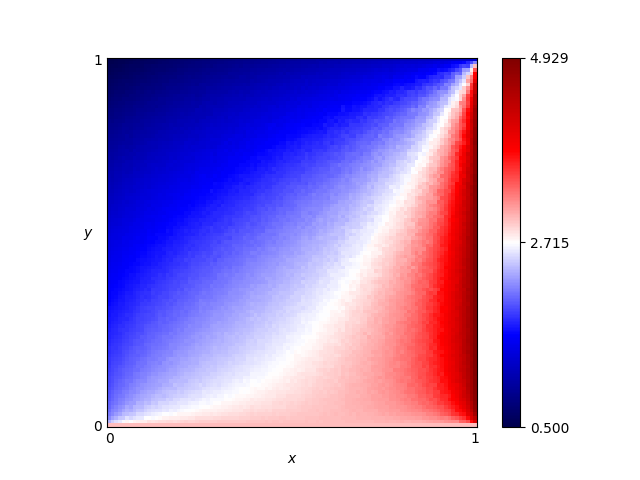
\includegraphics[height=.3\textheight]{./assets/images/Win-Stay_Lose-Shift.png}
    \caption{Pavlov fingerprinting with Tit for Tat used as the probe strategy.
    Figure was generated using~\cite{axelrodproject}.}
    \label{fig:fingerprinting}
\end{figure}

\subsection{Evolved strategies}

Complex strategies are defined as a set of strategies tha can use a variety of 
features computed from the history of play. The term complex can also be
refereed to strategies that have been trained with evolutionary methods to 
be dominant. In~\cite{Axelrod1987}, Axelrod used an evolutionary algorithm to 
identify a strategy that was equal to or better than Tit for Tat.

Other representation methods include lookup tables~\cite{Axelrod1987, Lindgren1994}
and artificial neural networks~\cite{Fogel1996, Lee2015}. In~\cite{Axelrod1987},
lookup tables are introduced as a mean of representing a strategy in a gene 
format. A lookup table is a set of deterministic responses based on the
opponents \(m\) last moves; \cite{Axelrod1987} considered \(m=3\).
Figures~\ref{fig:tit_for_tat_lu} shows a look up representation of Tit for Tat
where \(m=1\).

\begin{figure}[!hbtp]
    \centering
    \includestandalone[width=.25\textwidth]{./assets/tex/tit_for_tat_lu}
    \caption{Lookup table representation of Tit for Tat.}
    \label{fig:tit_for_tat_lu}
\end{figure}

Similarly, artificial neural networks provide a mapping function to an action
based on a selection of features computed from the history of play. A number 
of strategies based on artificial neural networks are introduced by~\cite{Knight2017}.
These strategies are refereed to as \textbf{EvovlvedANN} strategies and are
based on a pre-trained neural network with the following features,

\begin{multicols}{2}
    \begin{itemize}
        \item Opponent's first move is C
        \item Opponent's first move is D
        \item Opponent's second move is C
        \item Opponent's second move is D
        \item Player's previous move is C
        \item Player's previous move is D
        \item Player's second previous move is C
        \item Player's second previous move is D
        \item Opponent's previous move is C
        \item Opponent's previous move is D
        \item Opponent's second previous move is C
        \item Opponent's second previous move is D
        \item Total opponent cooperations
        \item Total opponent defections
        \item Total player cooperations
        \item Total player defections
        \item Round number
    \end{itemize}
\end{multicols}

A representation of \textbf{EvovlvedANN 5} is given in Figure~\ref{fig:ann_5_neural}. 
The inputs of the neural network are the 17 features as listed above. Number 5 
reefers to the size of the hidden layer.

\begin{figure}[!hbtp]
    \centering
    \includestandalone[width=.5\textwidth]{./assets/tex/ann_5_neural}
    \caption{Neural network representation of EvovlvedANN 5.}
    \label{fig:ann_5_neural}
\end{figure}

In~\cite{Knight2017}, these representing methods are refereed to as archetypes.
Finite state machines and artificial neural networks are included in the
work but also new archetypes are introduced, such as hidden Markov models. A variant
of a finite state machine that use probabilistic transitions based on the prior
round of play to other states and cooperate or defect with various probabilities
at each state. Finite state machines and hidden Markov models 
based strategies are characterized
by the number of states. Similarly, artificial neural networks based players
are characterized by the size of the hidden layer and number of input features.

Additionally a variant of a look up table is also presented called the lookerup 
archetype. The lookerup archetype responses based on the opponent's first \(n_1\)
moves, the opponent's last \(m_1\) moves, and the players last \(m_2\) moves.
Taking into account the initial move of the opponent can give many insights. 
For it is the only move a strategy is truly itself without being affected by
the other player. As a reminder, Axelrod in his work 
highlighted the importance of the initial move and believed that it was one
of the secrets of success of the strategy Tit for Tat.

Finally, a new archetype called the Gambler is also introduced, which is a 
stochastic variant of the lookerup archetype.

Archetypes are used with evolutionary algorithms to train set of 
new strategies. The evolutionary algorithm used in both~\cite{Axelrod1987,
Gaudesi2016} is called genetic algorithm. Other algorithms including particle
swarm optimization have been used in research of the most dominant strategy
\cite{Franken2005}.

In~\cite{Knight2017} the approach in used to introduce as stated
by the authors the best performing strategies for the iterated prisoner's dilemma.
These strategies will be refereed  as \textbf{Evolved} strategies.
Several successful new strategies are,

\begin{itemize}
    \item \textbf{EvolvedLookerUp2\_2\_2} a looker up strategy trained with a
    genetic algorithm; EvolvedLookerUp2\_2\_2 responses based on the opponent's 
    2 first and last moves and the player's 2 last moves. Thus \(n_1=2, m_1=2\)
    and \(m_2=2\). 
    \item \textbf{Evolved HMM 5} a 5 states hidden markov model trained with a genetic 
    algorithm;
    \item \textbf{Evolved FSM 16} a 16 state machine trained with a genetic
    algorithm; 
    \item Finally \textbf{PSO Gambler 2 2 2} a looker up strategy trained with
    a particle swarm algorithm, where \(n_1=2, m_1=2\) and \(m_2=2\).
\end{itemize}

Though several papers have claimed before to have discovered the dominant
strategies for the game the work of \cite{Knight2017} is promising. 
This is due the fact that the introduced strategies have been trained using
different types of evolutionary algorithms in a pool of 176 well known 
strategies for the literature. Including all the strategies that have been 
discussed in this section.

This was made possible due an open source  library, called the Axelrod project
\cite{axelrodproject}. The project is written in the programming language 
Python, it is accessible and open source. To date the list of strategies implemented
within the library exceed the 200. The project has been used in several
publications including~\cite{Knight2017} and a paper describing it and
it's capabilities was published in 2016~\cite{Knight2016}. The source code
for Tit for Tat as implement within the library is shown in Figure
\ref{fig:tit_for_tat_axelrod}. Furthermore, performing a tournament 
with a selection of strategies is possible in five lines of code, shown in 
Figure~\ref{fig:tournament_code}.

\begin{figure}[!hbtp]
    \centering
    \begin{minted}
        [
        autogobble=true,
        framesep=2mm,
        fontsize=\normalsize,
        ]
        {python}
def strategy(self, opponent: Player) -> Action:
    """This is the actual strategy"""
    # First move
    if not self.history:
        return C
    # React to the opponent's last move
    if opponent.history[-1] == D:
        return D
    return C
    \end{minted}
    \caption{\label{fig:tit_for_tat_axelrod} Source code for Tit for Tat in Python
    as implemented in Axelrod Python library~\cite{axelrodproject}}.
\end{figure}

\begin{figure}[!hbtp]
    \centering
    \begin{minted}
        [
        autogobble=true,
        framesep=2mm,
        fontsize=\normalsize,
        ]
        {python}
>>> import axelrod as axl
>>> players = (axl.Cooperator(), axl.Defector(), axl.TitForTat(), axl.Grudger())
>>> tournament = axl.Tournament(players)
>>> results = tournament.play()
>>> results.ranked_names
['Defector', 'Tit For Tat', 'Grudger', 'Cooperator']
    \end{minted}
    \caption{\label{fig:tournament_code} Performing a computer tournament
    using~\cite{axelrodproject}.}
\end{figure}
Software has a crucial role in research. Well written and maintained software
allows the reproducibility of prior work and can accelerate findings within the
field. The field of the iterated prisoner's dilemma has suffered the consequences
of poor research software. As stated above the source code of the initial
computer tournament is not retrievable. Several of the strategies that competed
in the tournament are not given a full explanation of how the decided on their
next move. In terms of best practice and reproducibility the Axelrod library
is the lead software in the field.

\subsection{Other Software}

Due the nature of the research regarding the iterated prisoner's dilemma
several software packages have been created in order to simulate computer
tournaments.

Another piece of software includes a library called PRISON~\cite{prison}.
PRISON is written in the programming language Java and it has been used by it's authors
in several publications. The project includes a good number of strategies from
the literature but unfortunately the last update of the project dates back in 2004.

More recent projects include~\cite{pd_trust, pd_game}, both are education 
platforms and not research tools. In~\cite{pd_trust}, several concepts such as 
the iterated game, computer tournaments and evolutionary dynamics are introduced
through a user interface game. Project~\cite{pd_game} offers a big collection of
strategies and allows the user to try several match and tournaments configurations.
Such as noise. 

\subsection{Applications}

\subsubsection{Social Applications}
%TODO include social studies. 

\subsubsection{Ecological Applications}

The reciprocal period of the prisoner's dilemma spread the knowledge of the
game not only worldwide but also across different scientific principles. The
study of cooperation was once again a critical issue. The applications of
the game soon found their way to ecological studies, for example 
\cite{Milinski1987} conducted an experiment using sticklebacks to test
the robustness of the strategy Tit for Tat in the interactions of fish. Fish usually
travel in pairs and monitor their hunters to gain information on the enemy.
Other works that include applications to ecological settings have been those
of~\cite{Godfray1992, Wilkinson1984}. There the reciprocal food sharing
between vampire bats was studied.

\subsubsection{Biological Applications}
%TODO include the cancer studies.
\begin{itemize}
    \item \cite{Turner1999} uses evolutionary game theory to study the spread of
    virus.
    \item \cite{Douglas2011} a shout for his work, using tit for tat to study cells.
\end{itemize}
\subsubsection{not sure}
In~\cite{Rapoport2015}, the authors claim that they have managed to 
re-run the first tournament that Axelrod performed. They tried to push his work
further by altering aspects such as, the format of the tournament, the objective
and the population. One of the authors claimed to have been a contributor
to the first tournaments, which would explain how it was managed to reproduce
the tournament.

\section{Analysis}\label{section:analysis}

In the progress of writing the literature new questions were raised; is it 
possible to analyse a literature timeline and what information can be gathered. 
To address this question, a data analysis of literature is performed using various
machine learning techniques. The data analysis is carried out on a data set which
contains meta data of academic articles on the research of the iterated prisoner's 
dilemma.

\subsection{Data Collection}

Academic articles are accessible through scholarly databases and collections.
In this work 5 different source have been used to collect metadata on articles
regarding the prisoner's dilemma. The sources that have been used was due the fact
that they have an open API. APIs are an application protocol interface which
allows direct access to the data base of a journal. Receiving articles from
academic journal's APIs include two faces.

\begin{enumerate}
    \item requesting;
    \item receiving answer;
\end{enumerate}

\begin{figure}[!hbtp]
    \begin{center}
    \includestandalone[width=.8\textwidth]{assets/tex/api}
    \end{center}
\end{figure}

Both the requesting url and the received xml differ for different journals.
The data collection is a crucial proceeder and we wanted to be automated. For
this reason an open source project was used called Arcas. Arcas is
a Python tool and made the data collection trivial. It works as a translator
between the user and the different APIs.

In order to collect the data several keywords had to be specified. The keywords
were checked to exists within the title or the abstract of an article and the 
keywords used are given by Table~\ref{table:search_keywords}. 

\begin{table}[!hbtp]
    \begin{center}
        \begin{tabular}{lll}
            \toprule
             & Keywords & \\
            \midrule
             1 &  prisoner's dilemma & \\
             2 &  prisoners dilemma  & \\  
             3 &  prisoners evolution & \\
             4 &  prisoner game theory & \\
             5 &  R Axelrod & \\
             6 &  memory one strategy & \\
             7 & tit-for-tat & \\
             8 & tit for tata & \\
             9 & zero determinant strategies & \\
            \bottomrule
        \end{tabular}
    \end{center}
    \caption{Keywords used in searching for articles.}
    \label{table:search_keywords}
\end{table}

The search managed to retrieve a total of 1128 articles. The total number
of articles within the data is 1170, 42 articles have been added manually.
Though Arcas retrieves several metadata on articles only features list on 
Table~\ref{table:result_set} the following are considered in this analysis.

\begin{table}[!hbtp]
    \begin{center}
        \begin{tabular}{lll}
            \toprule
             & Result name & Explanation \\
             \midrule
             1 & Abstract & The abstract of the article.\\ 
             2 & Author & A single entity of an author from the list of 
             authors of the respective article.\\ 
             3 & Date & Year of publication.\\ 
             4 & Journal & Journal of publication.\\               
             5 & Provenance & Scholarly database for where the article was 
             collected.\\                        
             6 & Title & Title of article.\\               
            \bottomrule
        \end{tabular}
    \end{center}
    \caption{Structure of data set. Contained results.}
    \label{table:result_set}
\end{table}

\subsection{Preliminary Analysis}

The provenance of the 1128 articles that have been collected manually is given 
by Table~\ref{table:provenance}. Within these articles a total of 2110 different
authors exist and 1140 articles. Several articles have been published to more 
than one journal. Still they are treated as individual records. Abstract and 
journals differ between entries of the same title.

More specifically, a total number of 470 articles have been collected from arXiv
and 317 from Springer journal. From IEEE 253 articles, and finally a small 
number have been contributed by Nature and Plos.

\begin{table}[!hbtp]
    \begin{center}
        \begin{tabular}{lll}
            \toprule
             & provenance \\
            \midrule
             IEEE &  253 \\
             Nature & 25 \\  
             PLOS & 63 \\
             Springer & 317 \\
             arXiv & 470 \\
            \bottomrule
        \end{tabular}
    \end{center}
    \caption{Keywords used in searching for articles.}
    \label{table:provenance}
\end{table}


In Figure~\ref{fig:provenance}, the number of articles collected per year
and per API are illustrated. Springer seems to have a continuous contribution on
the data set from 1996 up to 2017. The total number of articles collected from
Springer per year does not exceed 30. On the other hand, arXiv that has a 
significant contribution to the data set, seems to have articles on 
the iterated prisoner's dilemma a bit before the 2000s. Finally, PLOS
with a small significant contribution appears after 2005.

Additionally, the total number of articles per year have been plotted regardless
the provenance per year has been plotted in Figure~\ref{fig:timeline_no_points}.
This illustrates the time series. It is shown that there is a steady increase in
the number of articles until 2000 where a steep increase is spotted. There seems
to be a peak at the year of 2014 and a decrease from 2016 onwards.
That is due the fact that the latest data has been collected in November 2017.

\begin{figure}[!hbtp]
    \centering
    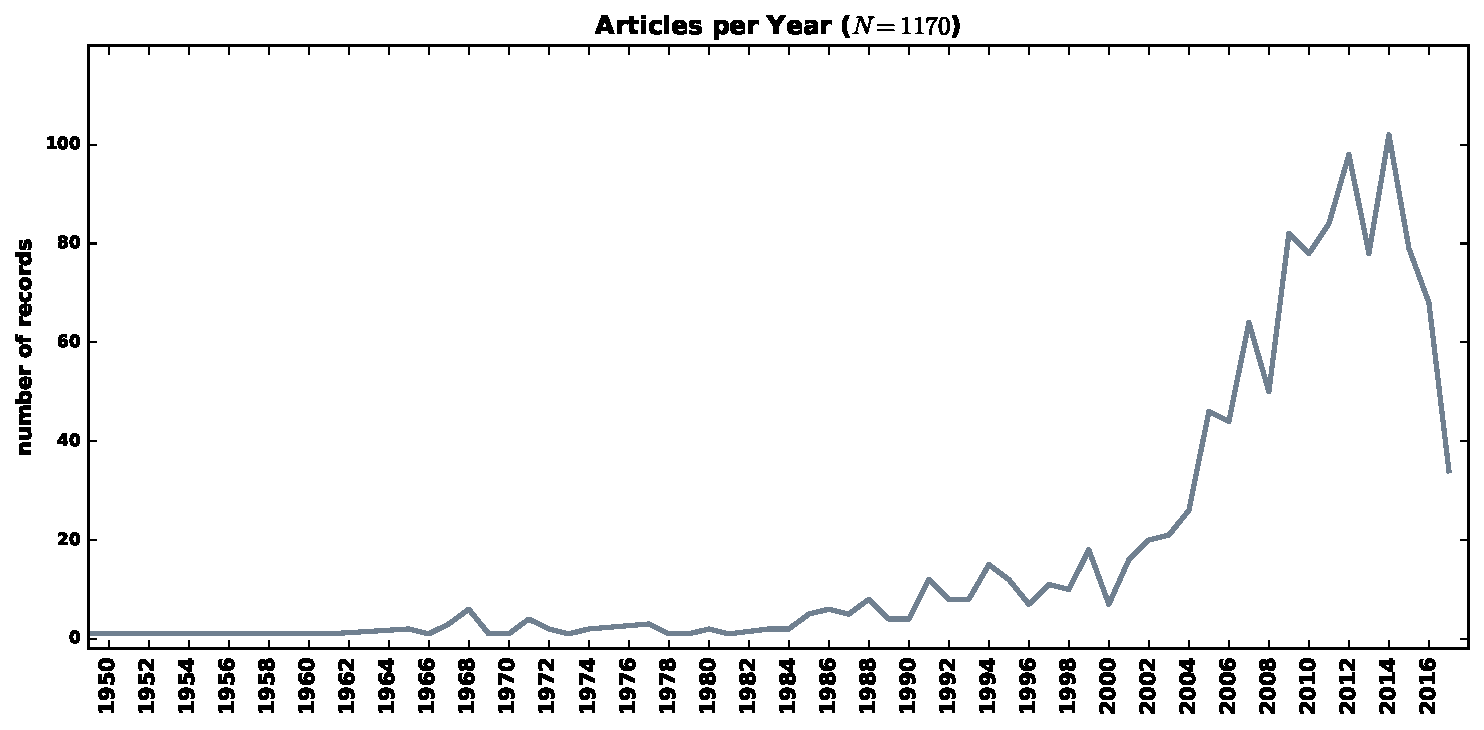
\includegraphics[width=.8\textwidth]{./assets/images/timeline_no_points.pdf}
    \caption{Provenance of articles}
    \label{fig:timeline_no_points}
\end{figure}

\begin{figure}[!hbtp]
    \centering
    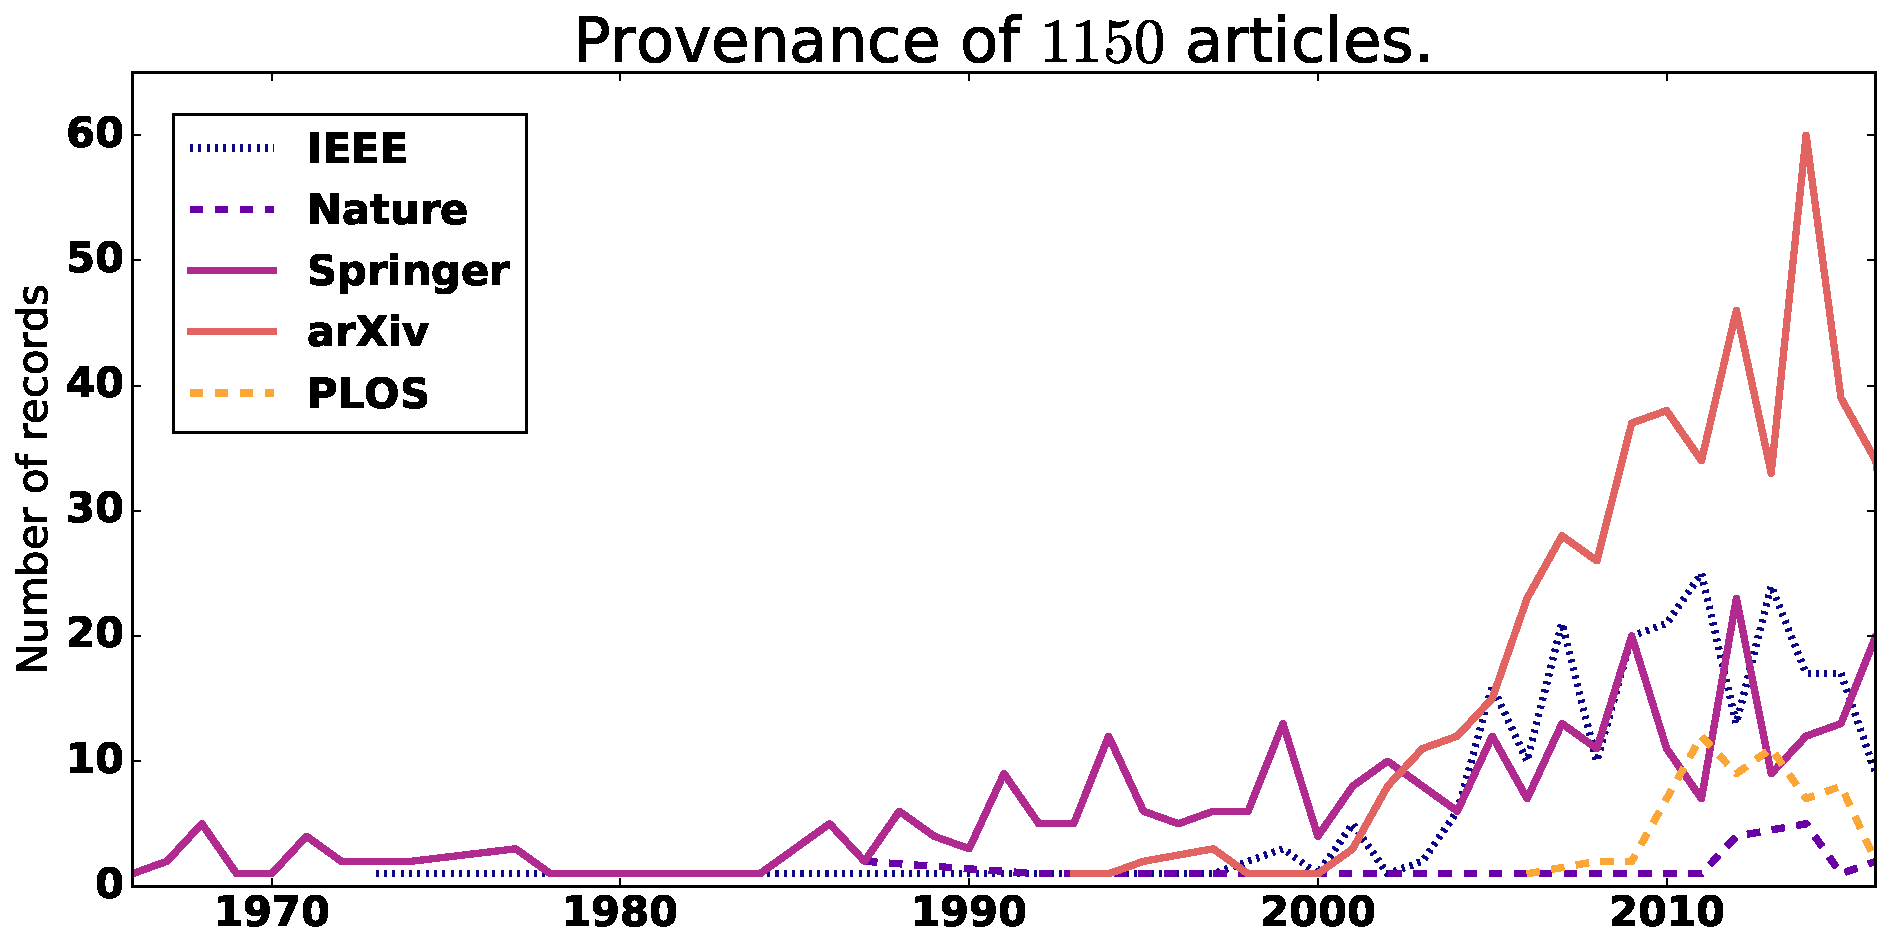
\includegraphics[width=.8\textwidth]{./assets/images/provenance.pdf}
    \caption{Provenance of articles}
    \label{fig:provenance}
\end{figure}

\subsection{Authors Analysis}
The data set contains a total of 2110 authors. Initially some the data were cleared.
Levenshtein Distance to calculate the differences between name entries. 
Interesting insights can be retrieved when looking at the co-authors links.
A graph has been generated where each node is an individual author, 
co authorships are the edges and weights are the number of times the authors 
have written together. 

The centrality of the network is looked upon. Betweeness unweighted, have been 
chosen as a centrality measure in this work. The results are given by Table
\ref{table:central_authors}.

\begin{table}[!hbtp]
    \begin{center}
        \begin{tabular}{lll}
            \toprule
            Name & Centrality \\
            \midrule
            Matjaz Perc & 0.0086 \\
            Yamir Moreno & 0.0073 \\
            Luo-luo Jiang & 0.0032 \\
            Arne Traulsen & 0.0031 \\
            Martin A. Nowak & 0.0030 \\
            V. Latora & 0.0028 \\
            Angel Sanchez & 0.0022 \\
            Krishnendu Chatterjee & 0.0021 \\
            Han-xin Yang & 0.0017 \\
            Zhihai Rong & 0.0015 \\
            \bottomrule
        \end{tabular}
    \end{center}
    \caption{Central authors.}
    \label{table:central_authors}
\end{table}

The immediate step is to look at the co-author cliques. A total of 
928 cliques exists within the graph and the max node number of a clique is 21.
For this work only the cliques with more than 5 authors is studied and from
those only the ones that.

\begin{figure}[!hbtp]
    \begin{subfigure}{0.3\textwidth}
        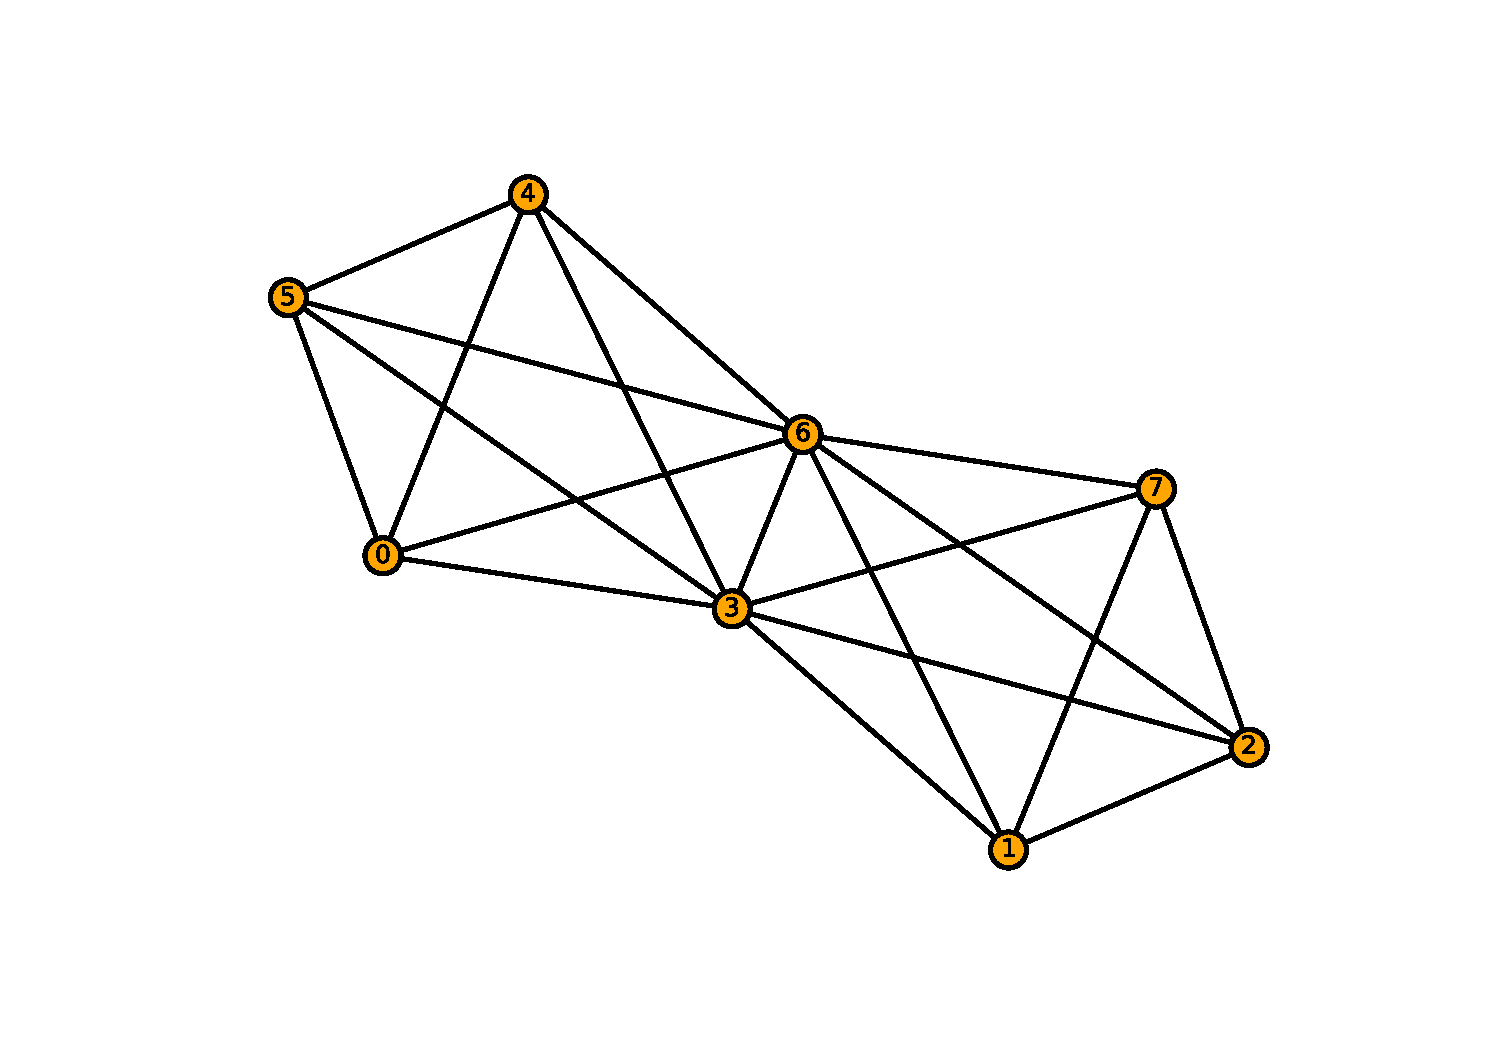
\includegraphics[width=\textwidth]{./assets/images/coauthor00.pdf}
    \end{subfigure}
    \begin{subfigure}{0.3\textwidth}
        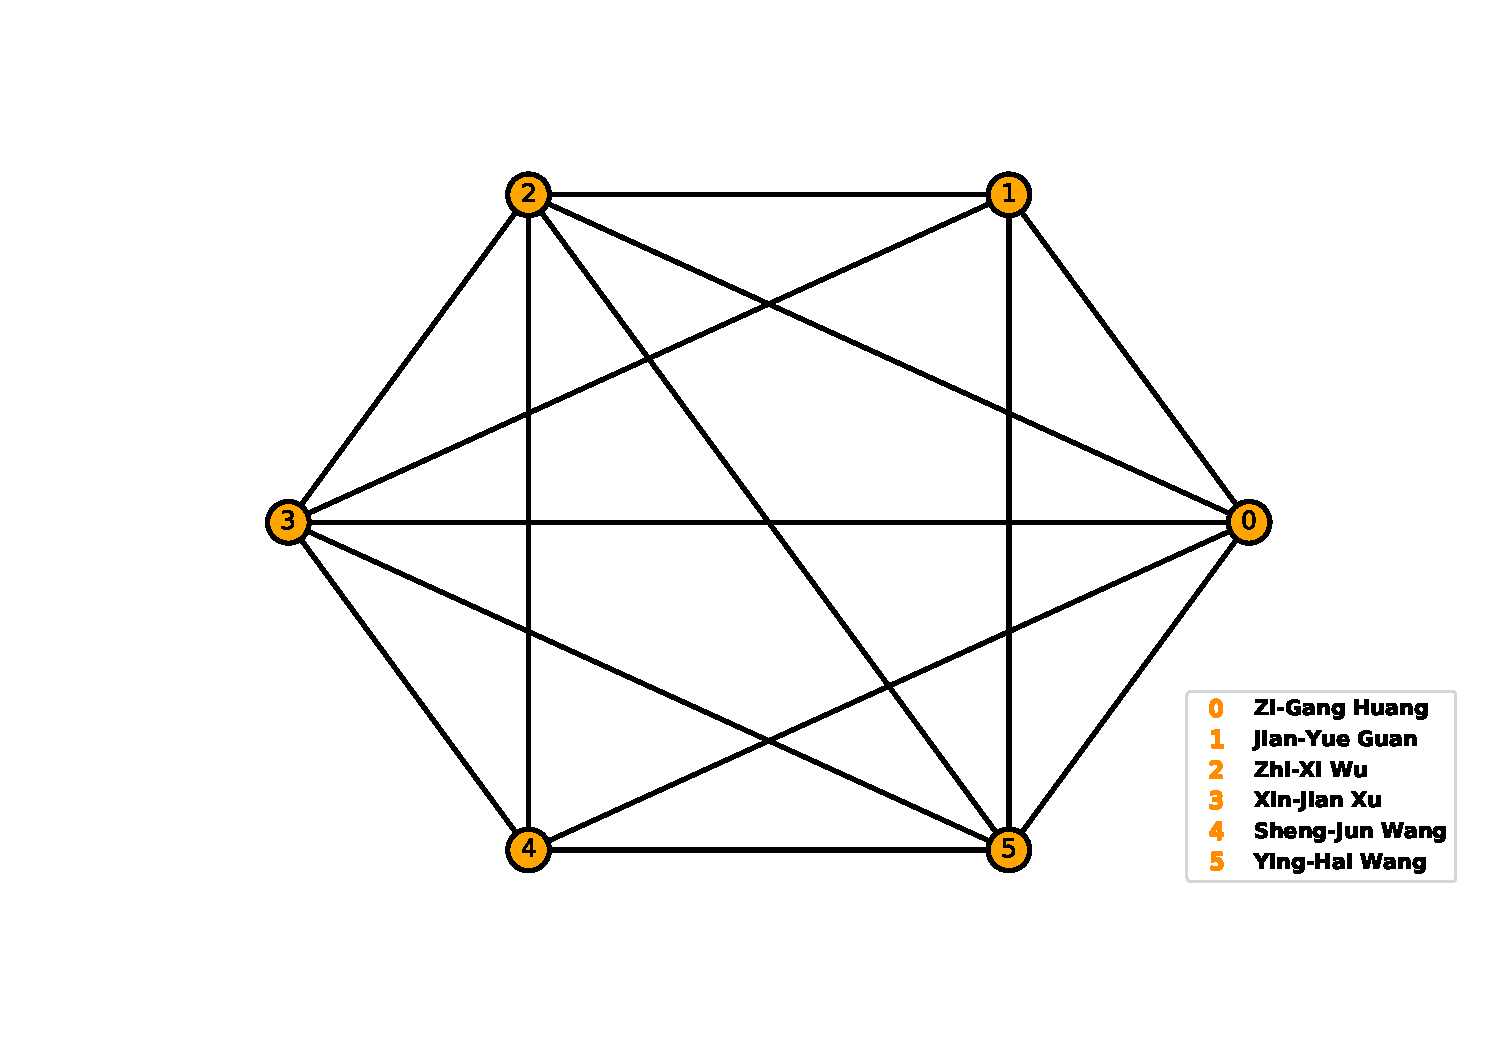
\includegraphics[width=\textwidth]{./assets/images/coauthor01.pdf}
    \end{subfigure}
    \begin{subfigure}{0.3\textwidth}
        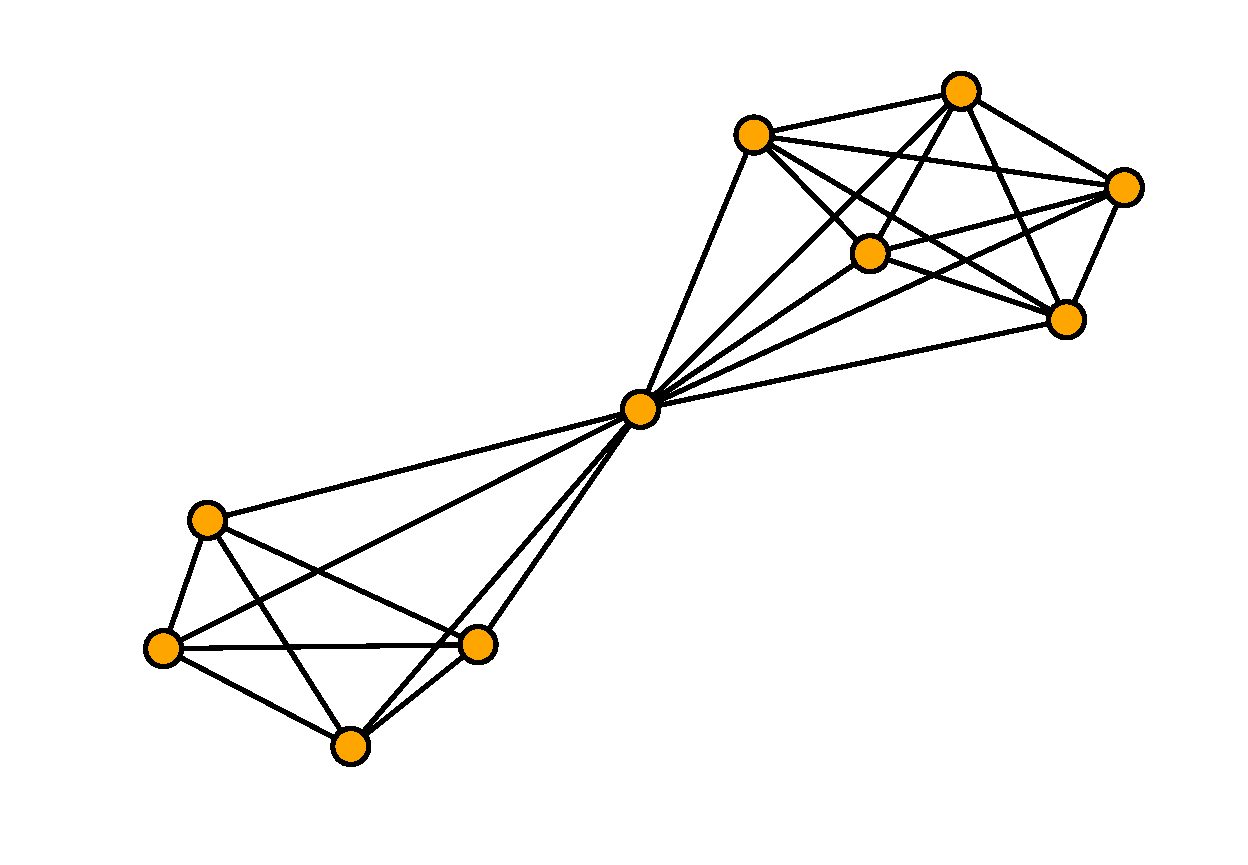
\includegraphics[width=\textwidth]{./assets/images/coauthor02.pdf}
    \end{subfigure}
    \begin{subfigure}{0.3\textwidth}
        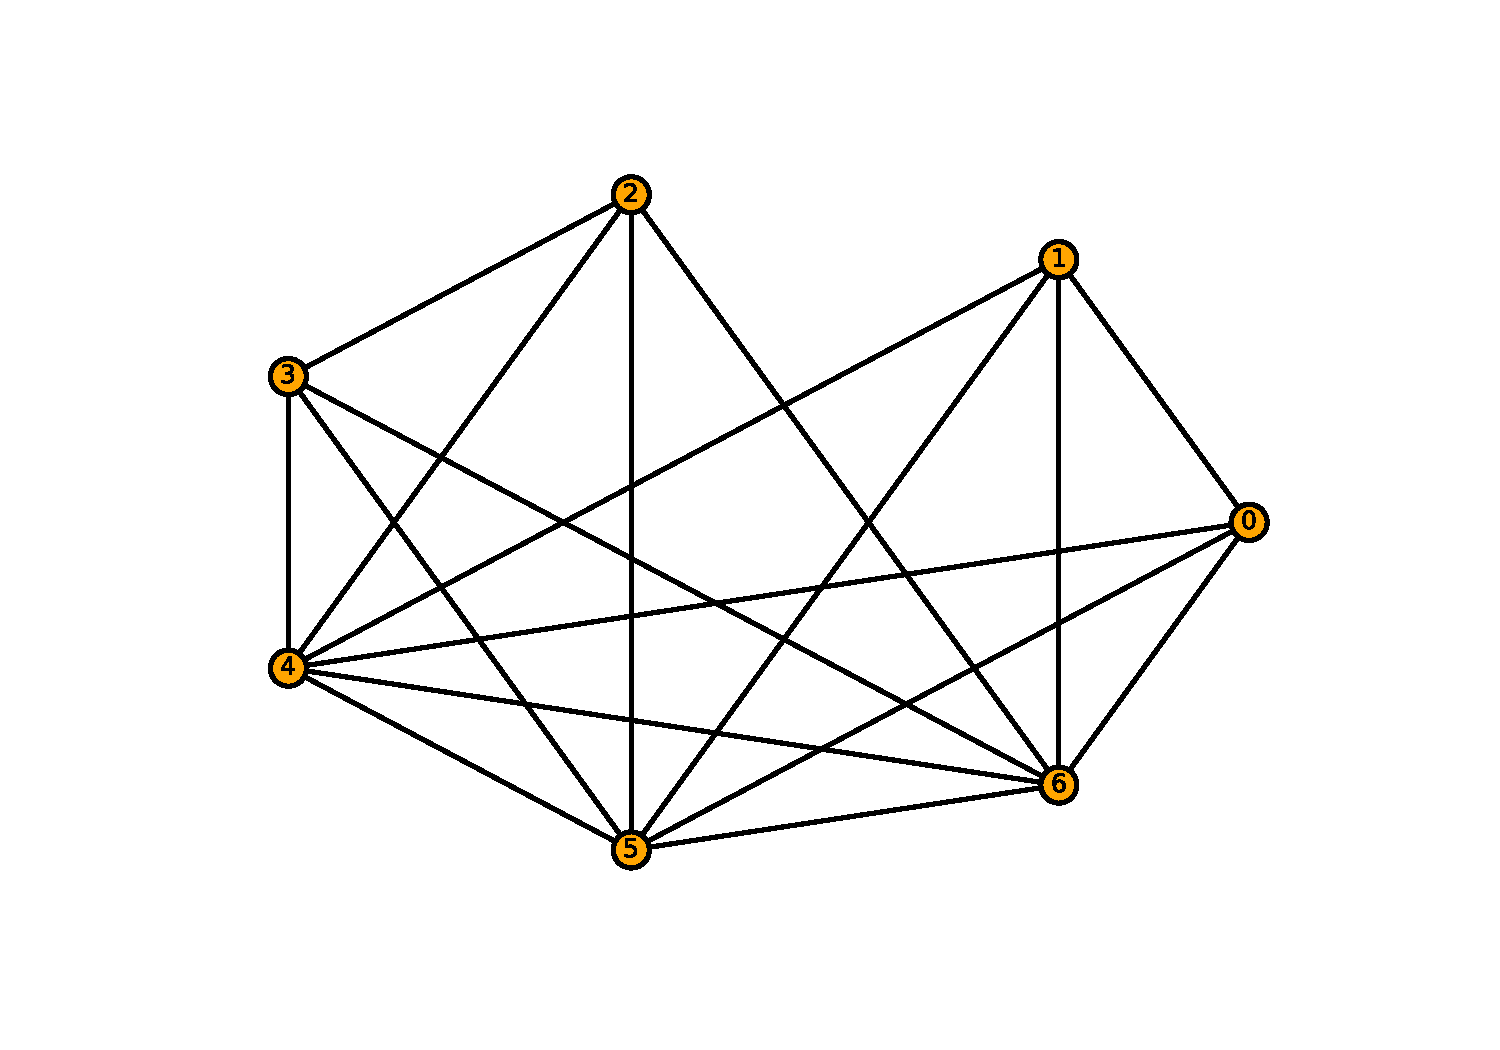
\includegraphics[width=\textwidth]{./assets/images/coauthor03.pdf}
    \end{subfigure}
    \begin{subfigure}{0.3\textwidth}
        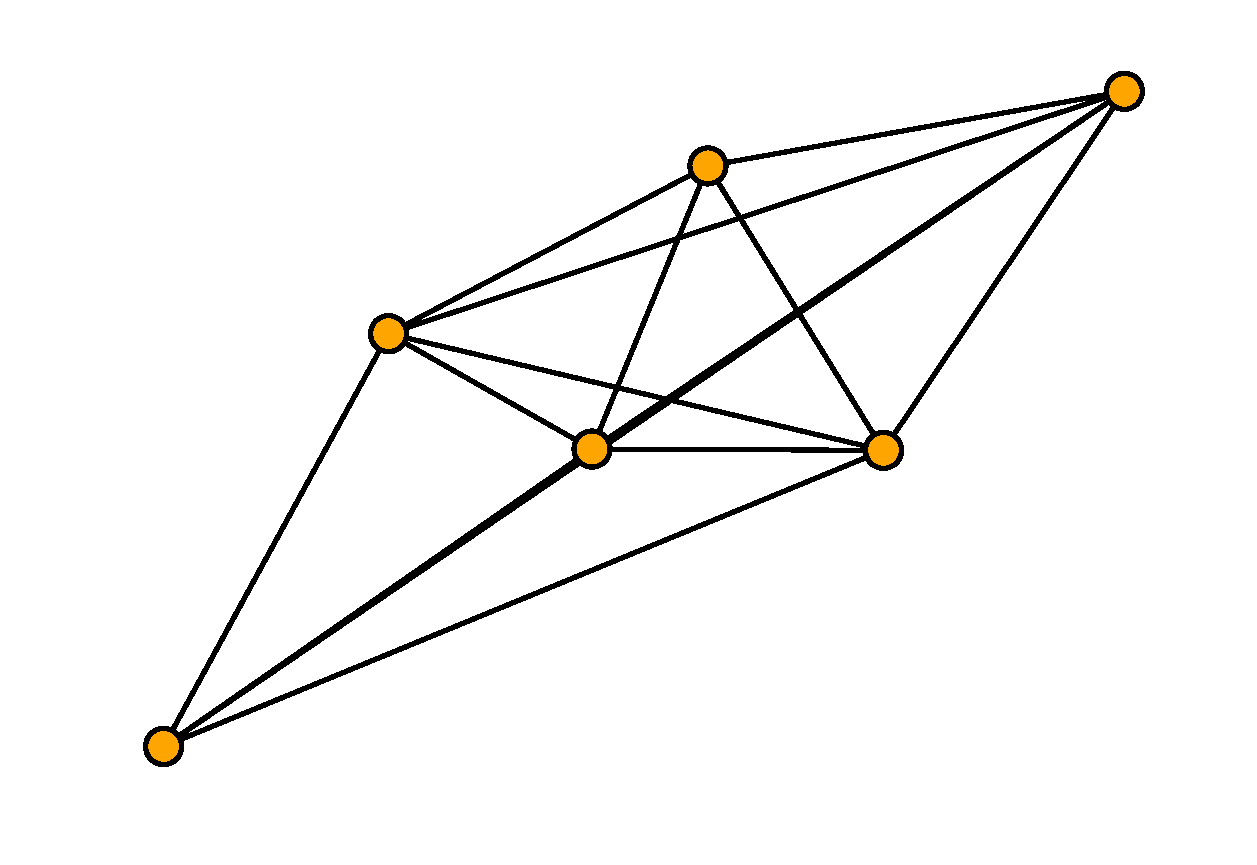
\includegraphics[width=\textwidth]{./assets/images/coauthor04.pdf}
    \end{subfigure}
    \begin{subfigure}{0.3\textwidth}
        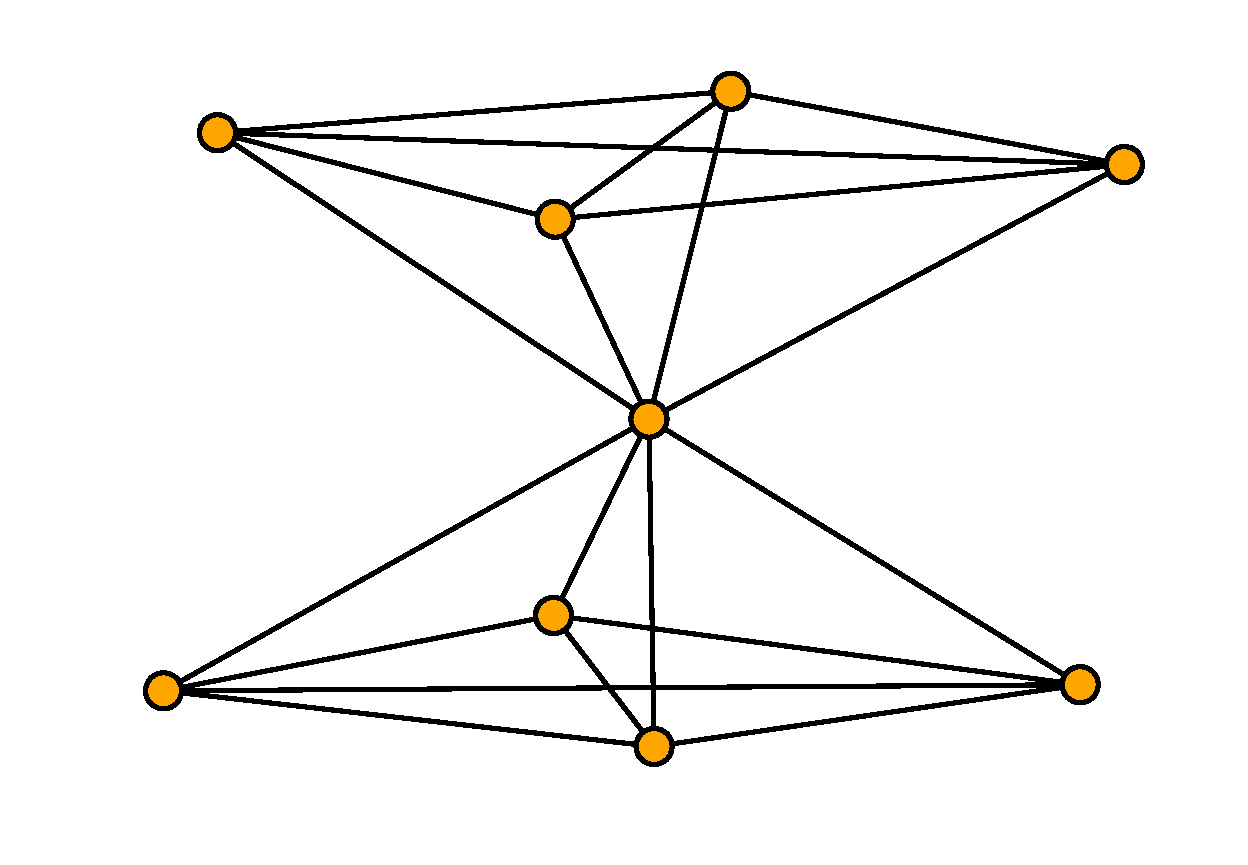
\includegraphics[width=\textwidth]{./assets/images/coauthor05.pdf}
    \end{subfigure}
    \begin{subfigure}{0.3\textwidth}
        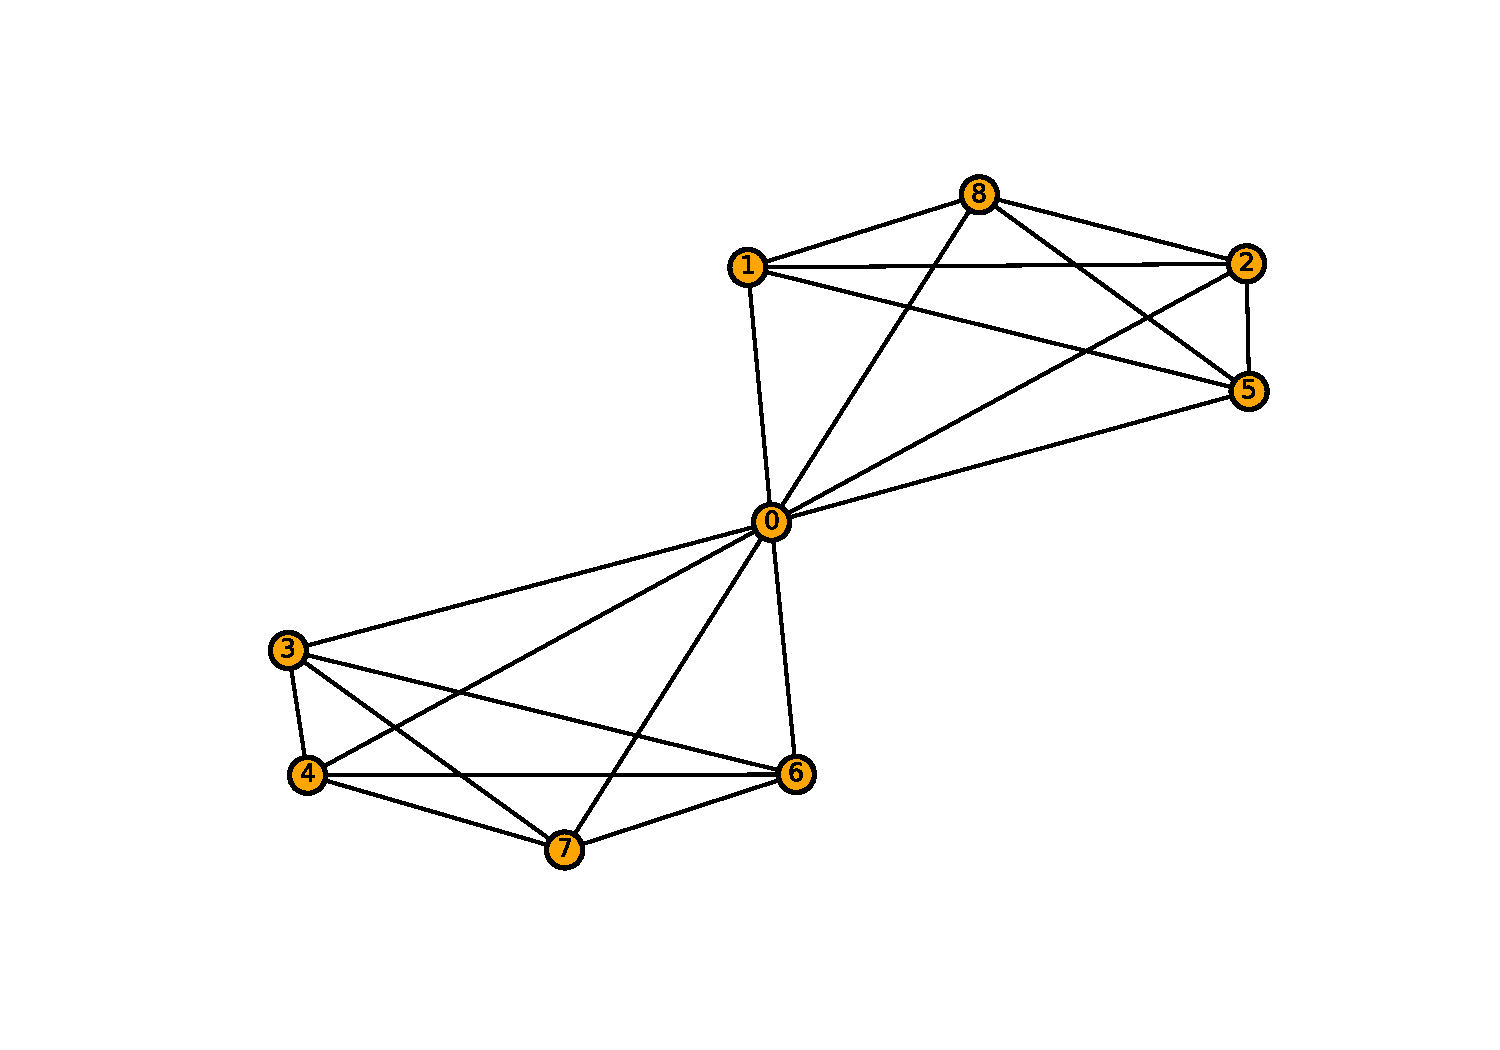
\includegraphics[width=\textwidth]{./assets/images/coauthor06.pdf}
    \end{subfigure}
    \begin{subfigure}{0.3\textwidth}
        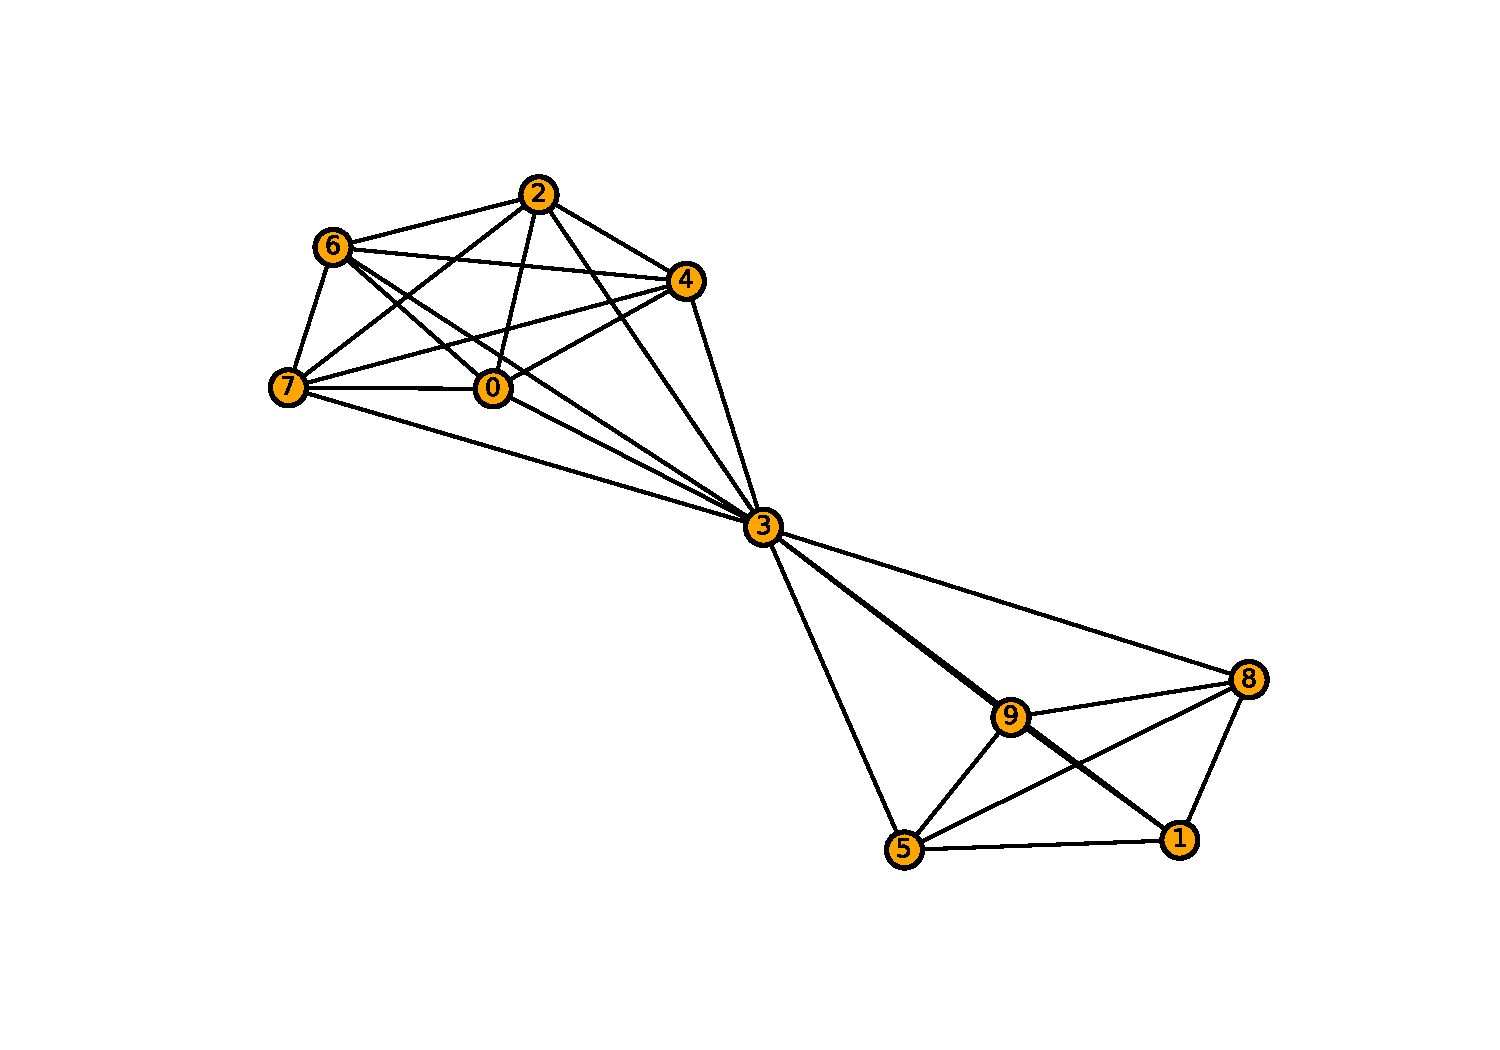
\includegraphics[width=\textwidth]{./assets/images/coauthor07.pdf}
    \end{subfigure}
    \begin{subfigure}{0.3\textwidth}
        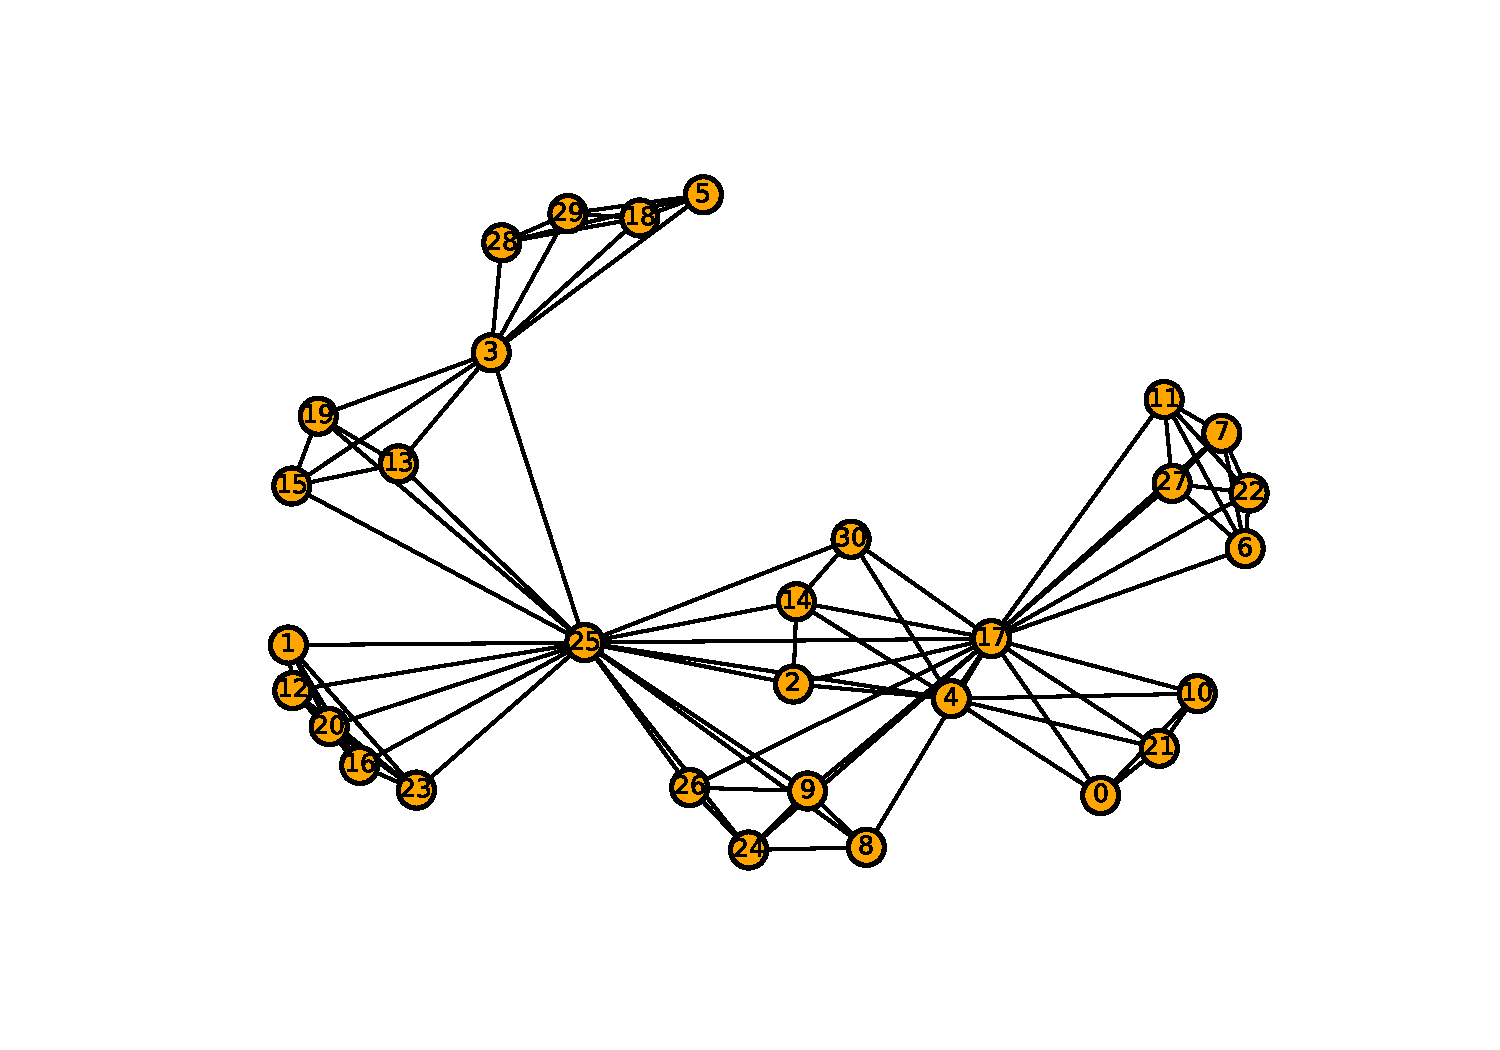
\includegraphics[width=\textwidth]{./assets/images/coauthor08.pdf}
    \end{subfigure}
\end{figure}

\bibliographystyle{plain}
\bibliography{bibliography.bib}
\end{document}